\chapter{Modelling User Location Preferences }
\label{chapter:Human location}
Domestic service robots in future should be able to gather knowledge about, the locations in the home where the user likes to spend time. Additionally, they should also know the time period when the users spend time in their favourite places. This acquired knowledge of the users location preference shall enable the robots to make informed decisions while assisting the user. For example, what time to clean a particular room or when to turn on the heater of the room. 

In this chapter, we focus on such \emph{knowledge acquisition} of user's location preferences based on spatio-temporal observations made by the robot. The user's location preferences can be defined as chances of finding a person at a locations at a particular time. Higher the preference, higher the chance of finding the person at that location. The advancement in long term autonomous navigation by \cite{krajnik_life-long_2015} and the rapid adoption of databases in the robots by \cite{niemueller2012generic}, has made the information collection for such knowledge generation possible in service robots. However even with these advancements there are some challenges which still needs to be addressed.  In more details, these challenges are  (i) modelling users location preference  (ii) prediction of users future locations  (iii) learning all these with sporadic observations made by the robots. 

Significant progress has been made by researchers in the field of human location behaviour, which is to learn the patterns in human location outdoors. Approaches for learning routine mobility  range from purely temporal  (\cite{mcinerney2013modelling, scellato2011nextplace}), spatial  (\cite{gao2012exploring,song2006evaluating}), to a combination  of  both   (\cite{eagle2009eigenbehaviors}). Non-parametric Bayesian methods are also gaining popularity given their ability to refine models as more data arrives. Chen et al.  (2012) used a Gaussian process to model congestion on road networks, while Gao et al.  (2012) used a hierarchical Pitman Yor process to model check-in behaviour on location-based social networks. Indoor human location behaviour was studied by \cite{krajnik_wheres_2015} using Fourier transform methods and Gaussian mixture models. 

While \cite{krajnik_wheres_2015}  work is first step towards learning human mobility behaviour in indoor environments, it failed to address the challenge of sparse dataset in domestic robots. As we have discussed earlier the observations on which the knowledge has to be learned, are sparse. We aim to demonstrate in this chapter that, by using Bayesian models, we can capture the human behaviour patterns in a sparse dataset.

We build Bayesian models which incorporate explicit domain knowledge and the structural knowledge about our data. Human behaviours are periodic in nature with a daily cycle. The models developed use this domain knowledge to extract the patterns emerging from the data caused by periodicity.

\section{Approach}

The robot while doing its activities, records the user's location it has detected in its robot memory along with the time and location as shown in Figure~\ref{fig:user_scan_human}. In ~\ref{tab:robot_record_human} the robot records if it recognizes a person along with its location and time .

  \begin{minipage}{\textwidth}
  \begin{minipage}[b]{0.49\textwidth}
    \centering
        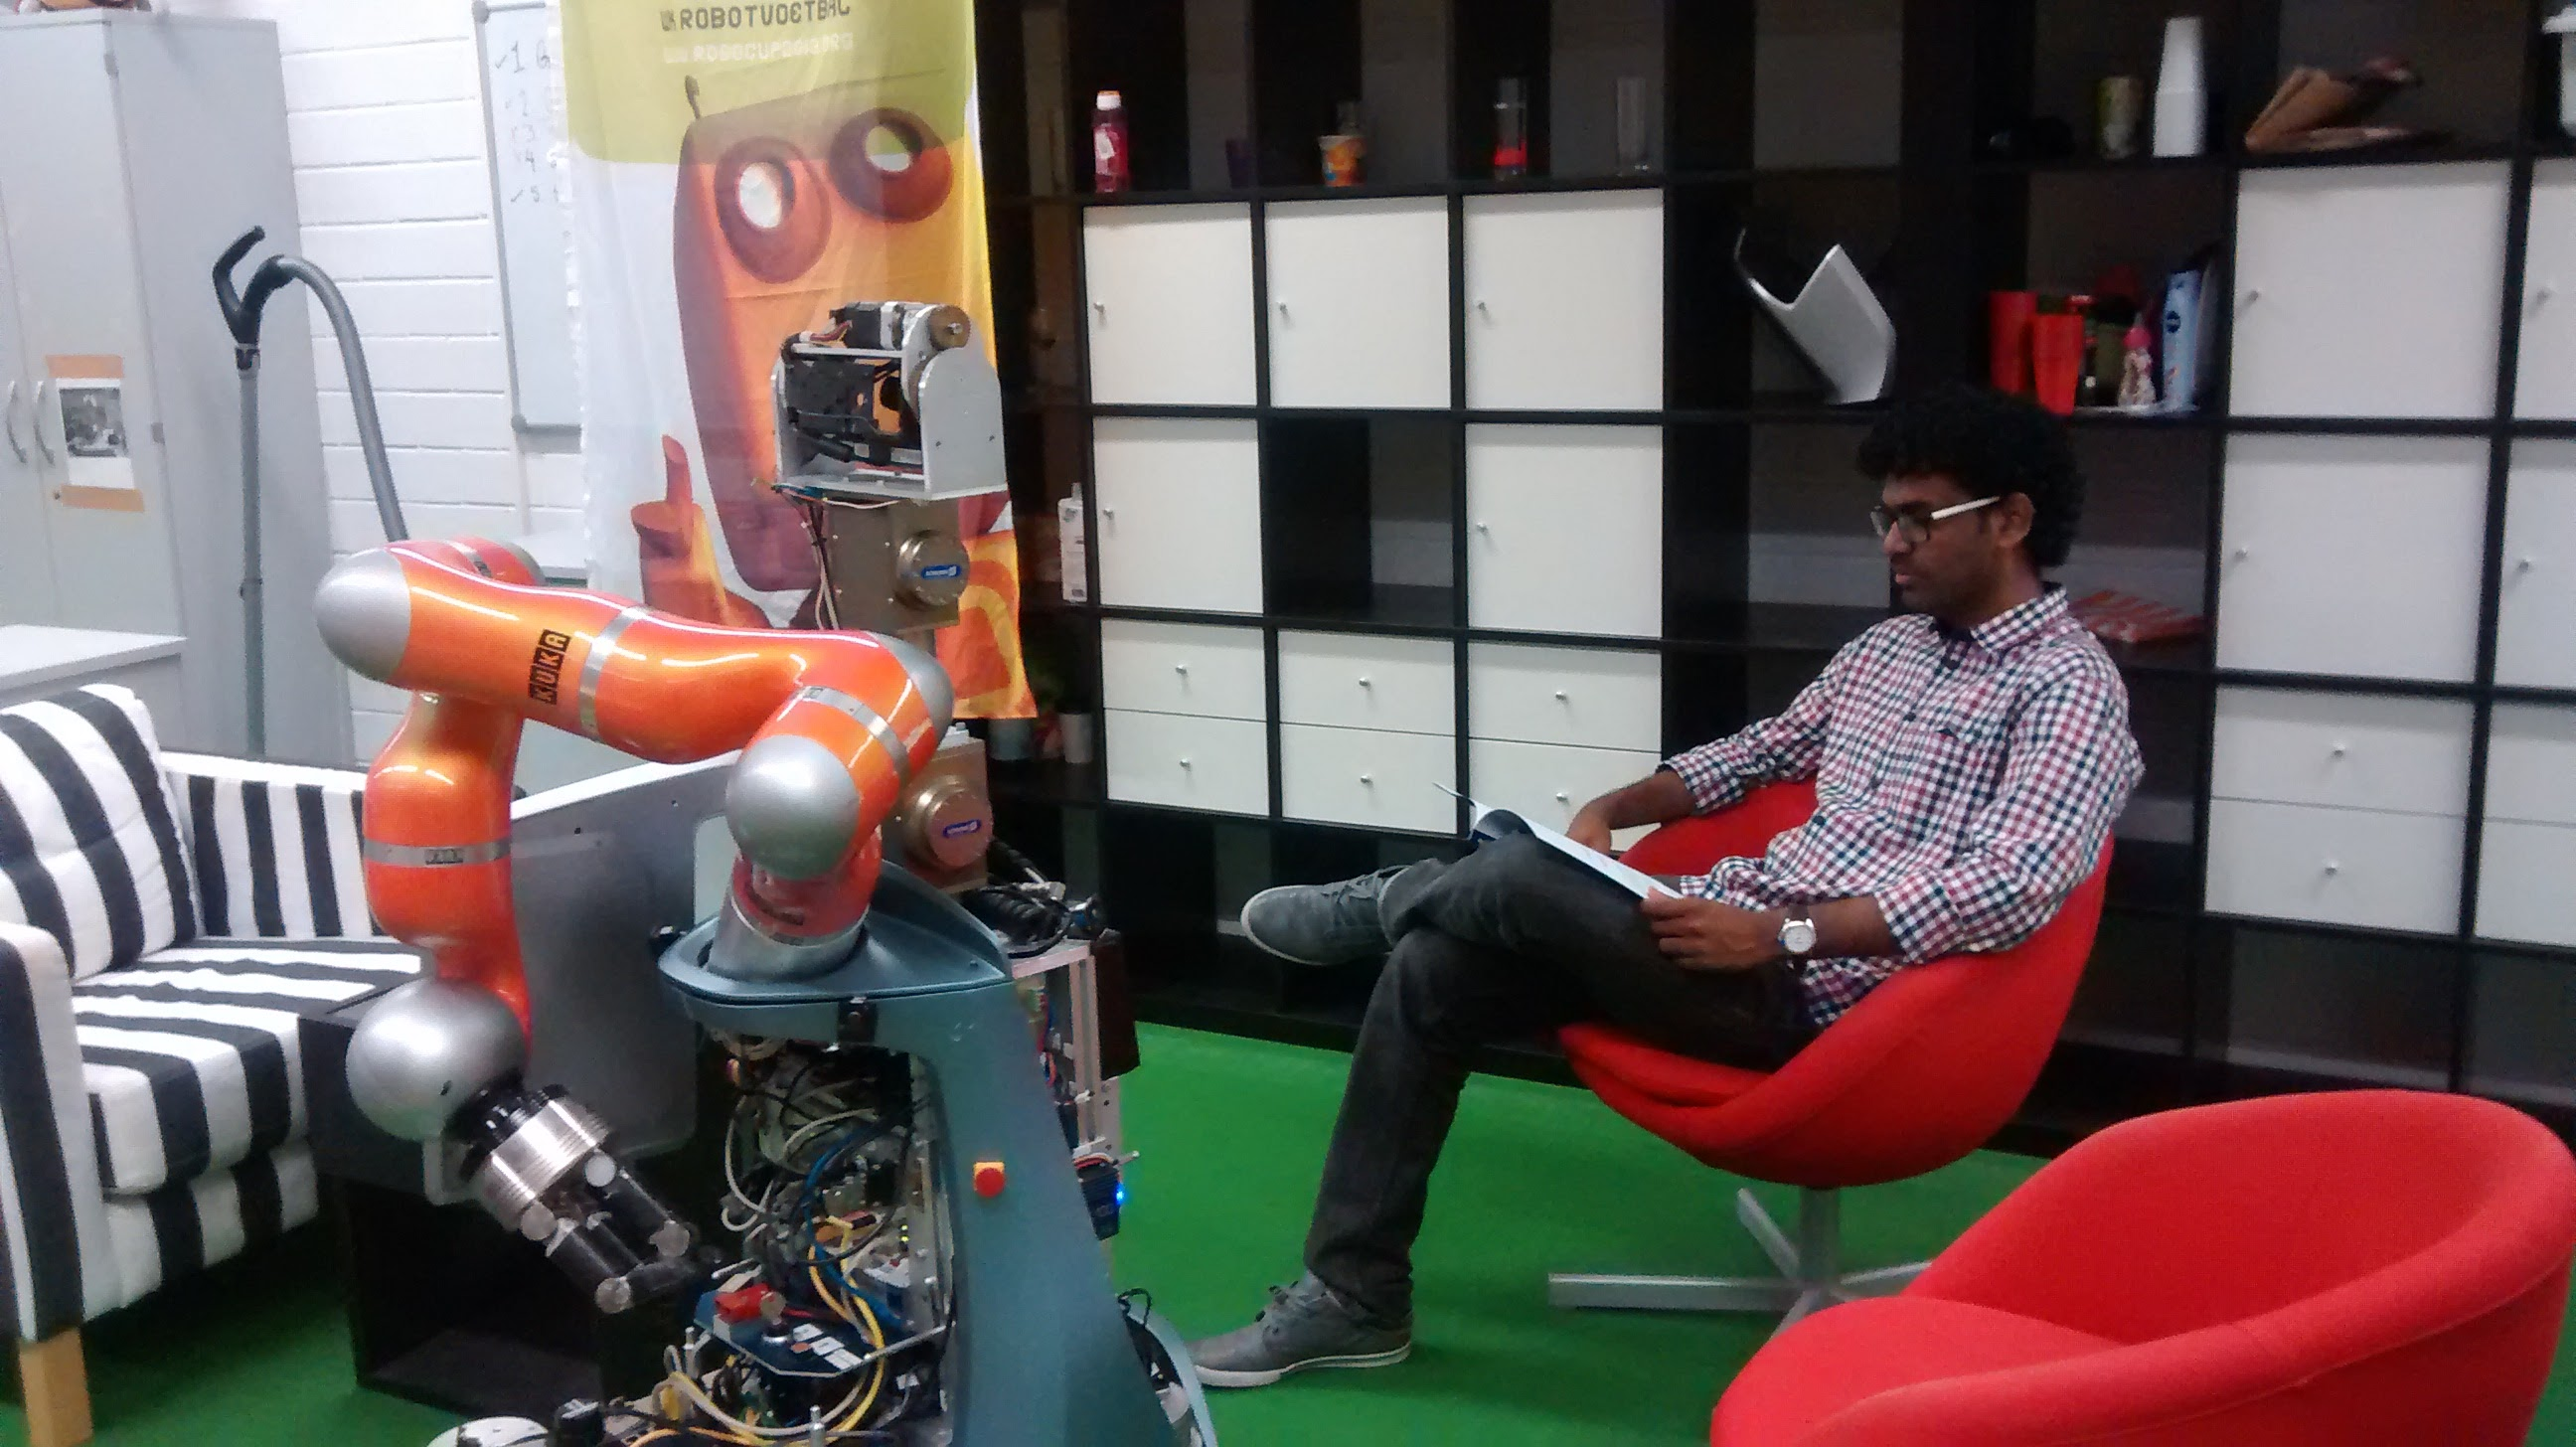
\includegraphics[width=0.9\textwidth]{images/cleaning_1.jpg}
    \captionof{figure}{Robot scanning living room}
    \label{fig:user_scan_human}
  \end{minipage}
  \hfill
  \begin{minipage}[b]{0.49\textwidth}
    \centering
    \begin{tabular}{|l|l|l|l|}
        \hline
	        Time & Person & Location \\
        \hline
        \hline
	        09.03 & Alice & kitchen \\
        \hline
	        09.34 & Deebul & living room \\
        \hline
	        10.05 & Bob & bathroom \\
        \hline
	        
        \end{tabular}
      \captionof{table}{Robot record human location}
      \label{tab:robot_record_human}
    \end{minipage}
  \end{minipage}

The model needs to model the ``Location" observation which is a nominal datatype. It can take different discrete values. As we know for modelling nominal variables we can use Categorical or Multinomial distribution. Since the data in our database comes sequentially, to enable on-line learning Categorical distribution is selected. Dirichlet distribution which is the conjugate prior of Categorical distribution, is selected as prior. These model is called Dirichlet Categorical model. Following sections will explain the generative model explanation.


\section{Dirichlet Categorical Model }

Dirichlet Categorical (DC) model  is a two-level Bayesian model. The basic idea is that observations of each time period is characterized by a distribution over the possible locations.

In chapter \ref{chapter: object} and \ref{chapter:occupancy} we learned the pattern in the user preferences of a single location. For modelling single location based on the presence and absence of data we used the Bernoulli distribution to quantify the preference. Here we would like to model the user preference over multiple locations in a single model. For modelling more than 2 discrete outcomes, we can use Categorical distribution. 

The data are the observed human location $x_{ij}$ for $i = 1 \dots T$ time periods and $j = 1, \dots , N$  are the observations.  We assume that the latent pattern in the persons location per period are distributed as a categorical distribution. The number of periods $T$ for our model is fixed to 24 corresponding to the number of hours in a day. 

The DC model is generalization of the Beta Binomial model to multiple classes of a categorical or multinomial distribution. The conjugate prior for the categorical distribution is the Dirichlet distribution. The model estimates the posterior distribution of $\theta_i$ given our current data and prior beliefs. Our prior beliefs are encoded in the model through the hyper-parameter $\alpha$, which represents  the robots belief on how the data should look like. Since we assume that the robot is learning from scratch we use to set of weak uniform beliefs. The probabilistic graphical model of  DCM is shown in Figure~\ref{dcm}

\noindent
\begin{figure}[htp]

\begin{minipage}{0.3\textwidth}
\centering

\tikz {
\node [const]                   (alpha) {$\alpha$};
\node [below=of alpha, latent]   (theta) {$\theta_i$};
\node [below=of theta, obs]      (x)     {$x_{ij}$};
\edge {alpha} {theta};
\edge {theta} {x};
\plate {trials} { (x)} {j location};
\plate {bags} { (theta) (x) (trials)} {i time};
}

\end{minipage}%
\begin{minipage}{0.7\textwidth}

\begin{equation*}
	\alpha = <1, 1, .... , 1 > 
\end{equation*}
\begin{equation*}
	\theta_i  \sim Dirichlet (\alpha)
\end{equation*}
\begin{equation*}
	x_{ij} \sim Categorical (\theta_i)
\end{equation*}
\end{minipage}
\caption[Dirichlet categorical graphical model representation]{Graphical model representation of DCM. The boxes are ``plates" representing replicates. The outer plates represents hours of a day, while the inner plate represents the choice of locations within each hour.}
\label{dcm}
\end{figure}

With the graphical model, the dependencies among the many variables can be captured concisely. The boxes are ``plates” representing replicates. The outer plate represents the hours of the day, while the inner plate represents the repeated choice of locations within each hour. Thus:

	$\alpha$ is  parameter of the dirichlet prior on per-period location distribution, 
	
	$\theta_i$ is the location distribution for period $i$  ,
	
	$x_{ij}$ is the observed location of the person in period $i$.
	
The $ x_{ij}$ are the only observable variables, and the other variables are latent variables. 

\section{Hierarchical Dirichlet Categorical Model}
\label{sec: HDCM}

Observations made only by a domestic robot using internal sensors and not using any external sensors creates the serious problem of sparsity. There are very much likely that some time periods there will be no observations available to learn. Maximum likelihood estimates of the categorical parameters assign uniform probability to the locations in these time periods. The standard approach to cope with this problem is to sharing statistical strength between time periods: it is as if the location we observe for each time period also provides weaker indirect location relevant to other time periods. In machine learning and statistical science this phenomenon is often called \emph{learning to learn} or \emph{transfer learning} \citep{kruschke2014doing}. Intuitively, knowing something about the location of person in the 9'o clock can help in gaining some information at 10'o clock. 

By placing a Dirichlet hyper-prior on the several Dirichlet parameter we obtain the  Hierarchical Dirichlet Categorical  (HDC) model. The hyper-prior makes it possible to share the learned knowledge from one prior to another. Thus learning about the location pattern at a higher level of abstraction helps to share it with the lower levels which have no observations.

The probabilistic graphical model of  hierarchical model is shown in Figure~\ref{hdcm}

\noindent
\begin{figure}[htp]

\begin{minipage}{0.3\textwidth}
\centering

\tikz {
\node [const]                    (alpha) {$\alpha$};
\node [below=of alpha, latent]   (beta)  {$\beta$};
\node [below=of beta, latent]    (theta) {$\theta_i$};
\node [below=of theta, obs]      (x)     {$x_{ij}$};
\edge {alpha} {beta};
\edge {beta} {theta};
\edge {theta} {x};
\plate {trials} { (x)} {j location};
\plate {bags} { (theta) (x) (trials)} {i time};
}

\end{minipage}%
\begin{minipage}{0.7\textwidth}

\begin{equation*}
	\alpha = <1, 1, .... , 1 > 
\end{equation*}
\begin{equation*}
	\beta \sim Dirichlet (\alpha)
\end{equation*}
\begin{equation*}
	\theta_i  \sim Dirichlet (\beta)
\end{equation*}
\begin{equation*}
	x_{ij} \sim Categorical (\theta_i)
\end{equation*}
\end{minipage}
\caption[Hierarchical dirichlet categorical graphical model representation]{Hierarchical Dirichlet Categorical Model. The boxes are ``plates" representing replicates. The outer plates represents hours of a day, while the inner plate represents the choice of locations within each hour.}
\label{hdcm}
\end{figure}

The model can be explained as:

	\boldmath{$\alpha$} is  constant Dirichlet prior for the hyperprior, 
	
	$\beta$ is a Dirichlet hyperprior,
	
	$\theta_i$ is the location distribution for period $i$  ,
	
	$x_{ij}$ is the observed location of the person in period $i$.
	
Thus we have categorical variables dependent on multiple priors sharing a hyperprior.


\section{Experiments}

We give an empirical performance analysis of the above models to determine their capabilities of learning user behaviour and preferences. We first conducted experiments on synthetic dataset to verify if the proposed models can learn and the number of observations required for making accurate predictions. Then we compare the DC and HDC models on their capabilities to learn using different observation size. Finally we evaluate the models predicting capabilities on a real dataset collected about human location in a home.

The goal of the experiments are to determine 
\begin{itemize}
	\item the robot is able to learn users location preferences.
	\item performance of HDC model compared to DC model.
	\item performance of HDC model with standard machine learning algorithms
	\item search time to locate a person.
\end{itemize}


\section{Model Learning Validation}

Before we start learning on the real dataset we want to validate the proposed models using a synthetic dataset. The synthetic dataset consists of observations generated using known ground truth probabilities. The models learn using the synthetic dataset and generate the learned probabilities. The distance between the learned probability and ground truth probability is used to quantify the learning of the model. 

\subsection{Simulated Dataset: User Location Dataset}

To demonstrate the learning in the proposed approach we have generated a user location dataset. The dataset consist of simulated observations of a user in a home environment made by a domestic robot \ref{fig:eval_human}. The robot can scan 4 locations in the home: A, B, C and D. The time of the scan is discretized into 3 times of the day: morning, afternoon and night. 

The generative process for each possible observation in the dataset 
\begin{itemize}
    \item Randomly choose $ \theta \sim Dirichlet (\alpha)$  (Distribution of user over location-time)
    \item Choose randomly the time period $i$.
	\item Choose the location $x_n$ $\sim$ Categorical$ (\theta_i)$ , where the user was observed.
	\end{itemize}

Ground truth of the Dirichlet distribution, signifying the user location distribution over time in shown in Figure \ref{fig:eval_user_gt}. The Dirichlet is the latent parameter to be learned by the robot.   The figure represents the hinton plot of the underlying Dirichlet distributions. Hinton plot are a way of visualizing probabilities. The size of the white square in the plot quantifies the belief of the probability. Higher the size of the box higher the probability. Thus for probability 1 we have a complete white box and gray means 0 probability. In the ground truth probability in Figure \ref{fig:eval_user_gt} the each row represents the distribution of the user at the particular time period. We see a big white box at location:D and time:night on the bottom left of the plot, while all other boxes for row night are comparatively small. This signifies that the user is more likely to be found in the at location D in the night than other places.  We evaluate our models on the observations generated from this distribution.

\begin{figure}
    \centering
    \begin{subfigure}[b]{0.4\textwidth}
        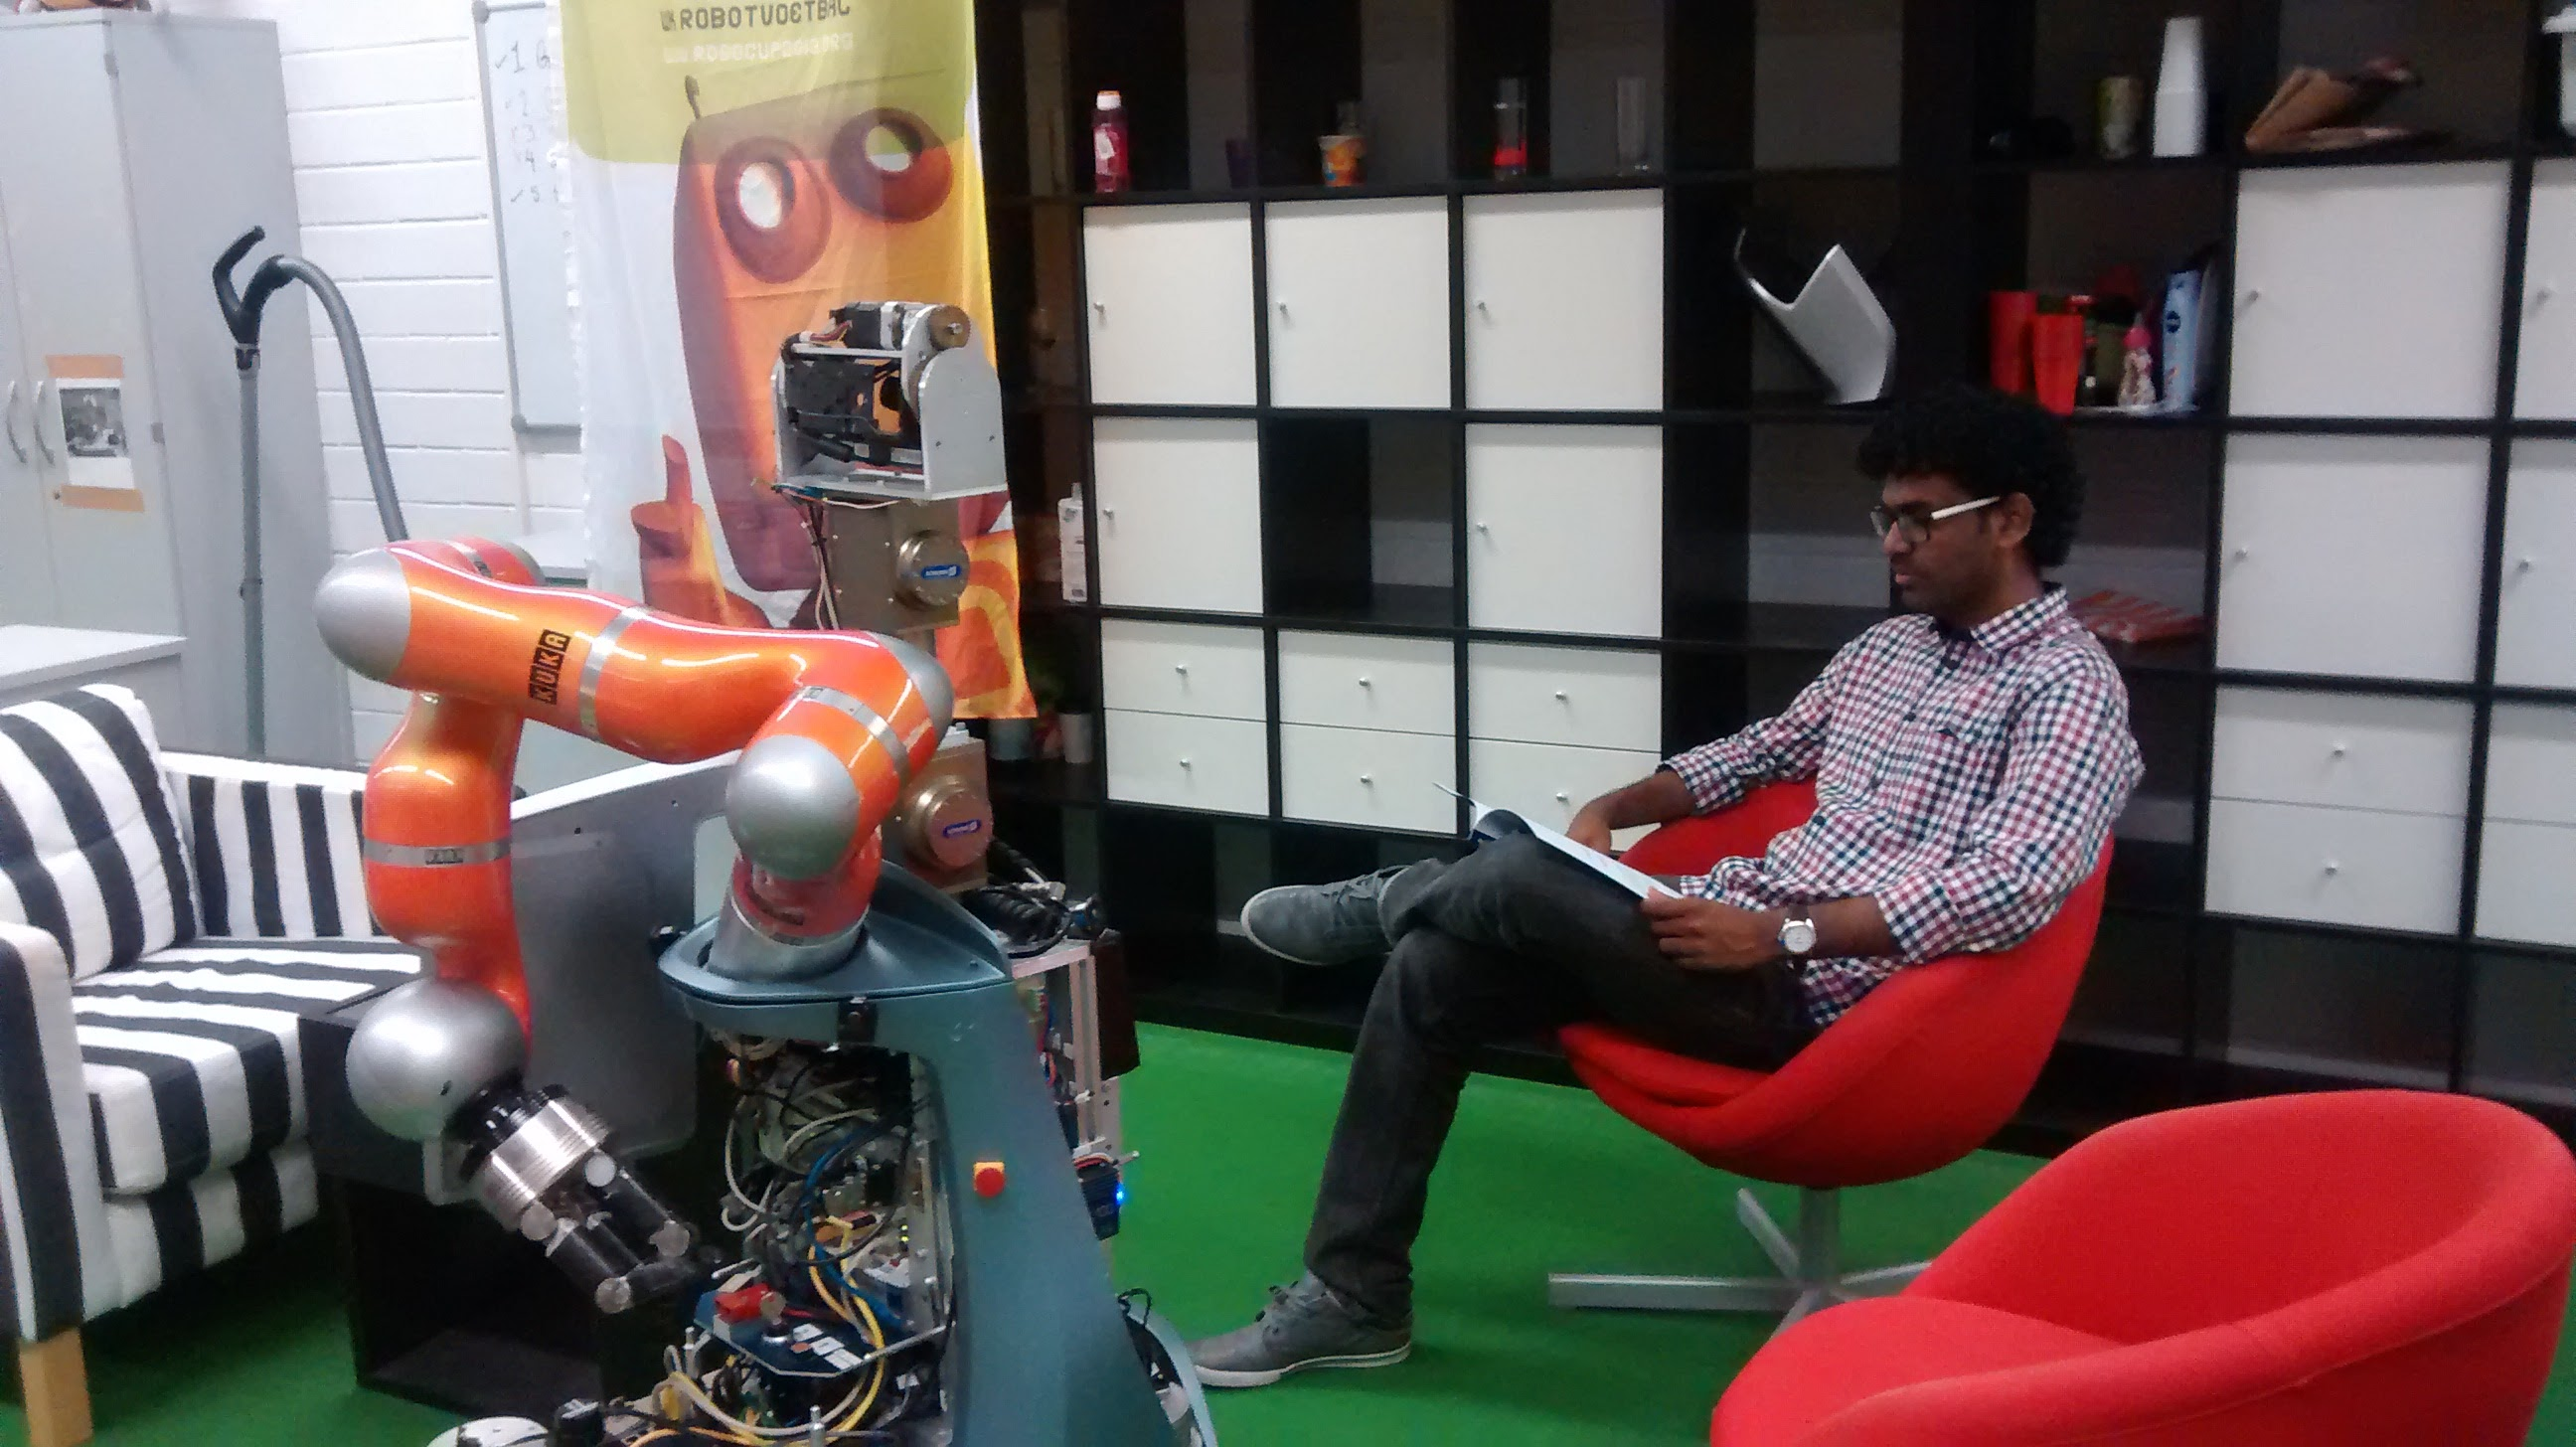
\includegraphics[width=\textwidth]{images/cleaning_1.jpg}
        \caption{}
        \label{fig:eval_human}
    \end{subfigure}
    ~ %add desired spacing between images, e. g. ~, \quad, \qquad, \hfill etc. 
      % (or a blank line to force the subfigure onto a new line)
    \begin{subfigure}[b]{0.4\textwidth}
        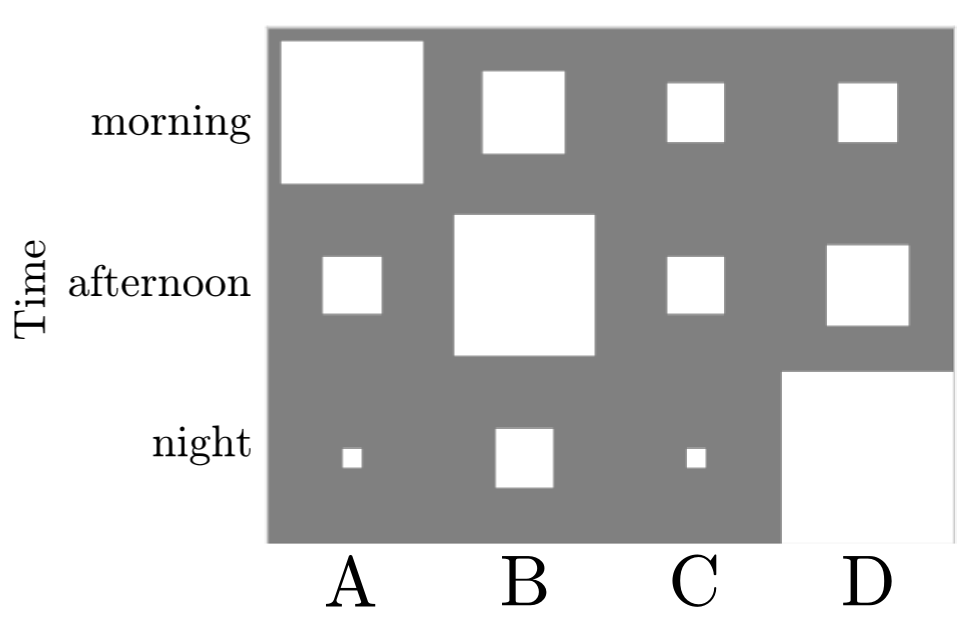
\includegraphics[width=\textwidth]{images/abc.png}
        \caption{}
        \label{fig:eval_user_gt}
    \end{subfigure}
    \caption[Model validation dataset generation]{Simulated dataset generation of the user location at different times of the day. (b) Simulated object locations ground truth probability distribution.
The x-axis represents the locations the y axis represents the time of observation. The size of the white box indicates the probability of the user presence at a particular time period.}
\label{}
\end{figure}




\subsection{Posterior Probability Check}
The first method is to visually compare the learned posterior probabilities with the ground truth.  In Figure~\ref{fig:eval-user-dc-hdc}, we can visually analyse the difference between the learned models of both DC model and HDC model. The leftmost plot \ref{fig:eval_user_2} as explained above is the ground truth probabilities from which the observations were generated. We generated a dataset with \textbf{100} observations. The models use the observations and infers its posterior distribution. The middle plot \ref{fig:eval-user-dc} is the learned posterior probabilities using the DC model while the last plot \ref{fig:eval-user-hdc} is the posterior probabilities using the HDC model. 

Visually we can observe from the plots both the posterior probabilities of both the models are similar to the ground truth probabilities. Thus we can conclude that the proposed models are converging to the true probabilities. In the next section we quantitatively compare the models using different data size.

\begin{figure}
    \centering
    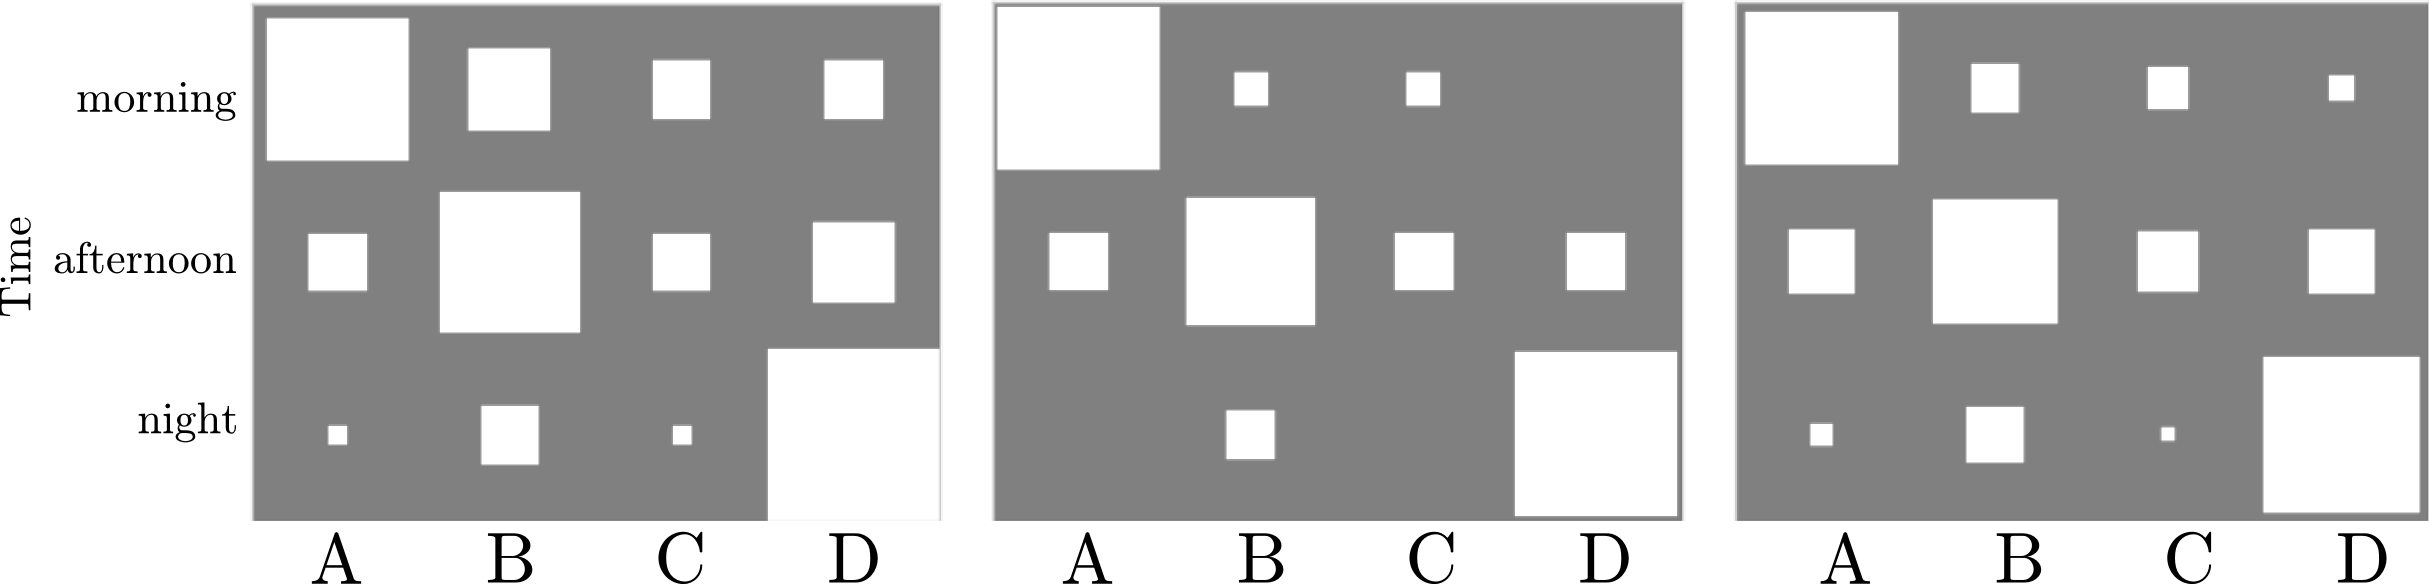
\includegraphics[width=\textwidth]{images/eval_human_results.png}
       
    \begin{minipage}[t]{.35\textwidth}
    %\centering
    \subcaption{Ground Truth}\label{fig:eval_user_2}
    \end{minipage}%
    \begin{minipage}[t]{.3\textwidth}
    %\centering
    \subcaption{DC model}\label{fig:eval-user-dc}
    \end{minipage}
    \begin{minipage}[t]{.25\textwidth}
    %\centering
    \subcaption{HDC model}\label{fig:eval-user-hdc}
    \end{minipage}

\caption[Posterior probabilities of DC and HDC ]{Posterior probabilities of the models : (a) is ground truth of the distribution. (b) is the learned distribution using the DC model. (c) is the learned distribution using the HDC  model . The x-axis represents the locations the y axis represents the time periods. The size of the white box indicates the probability of the user presence }\label{fig:eval-user-dc-hdc}
    
\end{figure}

\section{Model Comparison}

The goal of the experiments is to empirically validate the learning in both Dirichlet-Categorical and Hierarchical-Dirichlet-Categorical model 
learning using different data size. We also validate that HDC can compensate  for lack of observations in some time period by sharing information.

We use two metrics, for evaluating the performance of the developed models on the synthetic dataset. We use the adopted Bhattacharyya distance \cite{bhattacharyya1946measure} and Kullback–Leibler divergence \cite{kullback1951information}  (KL Divergence)to quantify the distance between the simulated and the learned Dirichlet distribution.   

\subsection{Bhattacharyya Distance}
Bhattacharyya distance measures the similarity of two discrete or continuous probability distributions. The distance ranges from 0 to $\infty$, with \textbf{0} meaning both probabilities are identical. The  adopted Bhattacharyya distance \cite{rauber2008bhattacharyya} for comparing dirichlet distributions is given by :
\begin{multline}
	D_B (Dir_a (x_1, \dots ,x+n), Dir (y_1, \dots , y_n)) = \nonumber\\
	 \Gamma \Bigg ( \frac{1}{2}  \sum_{i \in {1, \dots, n}} x_i +  \frac{1}{2}\sum_{i \in {1, \dots, n}} y_i\Bigg) + 
	\frac{1}{2}  \sum_{i \in {1, \dots, n}} \Gamma  (x_i) + 
	\frac{1}{2}  \sum_{i \in {1, \dots, n}} \Gamma  (y_i) - \\ 
	\sum_{i \in {1, \dots, n}} \Gamma \bigg (\frac{1}{2}  (x_i + y_i) \bigg) - \frac{1}{2}  \Gamma \Bigg (  \sum_{i \in {1, \dots, n}} x_i \Bigg) + \frac{1}{2}  \Gamma \Bigg ( \sum_{i \in {1, \dots, n}} y_i\Bigg)
\end{multline}

\subsection{Kullback–Leibler Divergence}
Similarly KL divergence also measures the similarity of two discrete or continuous probability distributions. Even for KL divergence, 0 signifies both probabilities are identical.  
The KL divergence between two distributions $p$ and $q$ is given by
\begin{equation*}
	KL (p||q) = \int p (x) \log \frac{p (x)}{q (x)} dx = \left < \log \frac{p (x)}{q (x)}  \right>_{p (x)}
\end{equation*}

Lets suppose we have two Dirichlet distributions $p$ and $q$ with parameters $\alpha$ and $\beta$ respectively, then the KL divergence between Dirichlet distributions\cite{kurt2013} is given by
\begin{equation*}
	\begin{split} 
 KL (p||q) &= \log \Gamma (\alpha_0) - \sum_{k=1}^K \log \Gamma (\alpha_k)   
 - \log \Gamma (\beta_0) \\ &+ \sum_{k=1}^K \log \Gamma (\beta_k)  + \sum_{k=1}^K  (\alpha_k – \beta_k)  (\psi (\alpha_k)-\psi (\alpha_0)) 
\end{split}
\end{equation*}


The only difference being that KL divergence is unsymmetrical while Bhattacharyya distance is symmetric. 

\subsection{Results}
We generated dataset with increasing number of observations from 20 to 800. For each observation set we trained both the models DC and HDC. Their corresponding distances with the ground truth were recorded. The process was repeated 100 times for each observation set.

\begin{figure}[htp]
\centering

\begin{subfigure}{.45\textwidth}
  \centering
  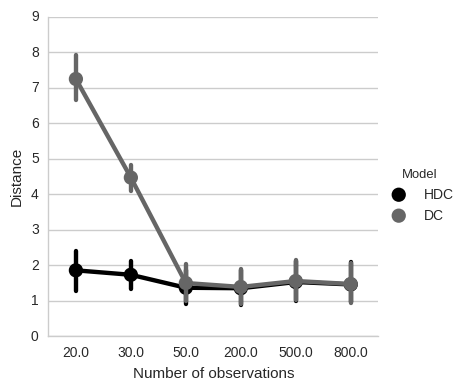
\includegraphics[width=\linewidth]{images/Eval-HDC-Bhattacharya-Distance.png}
    \caption{Bhattacharyya distance}
\end{subfigure}
\begin{subfigure}{.45\textwidth}
  \centering
  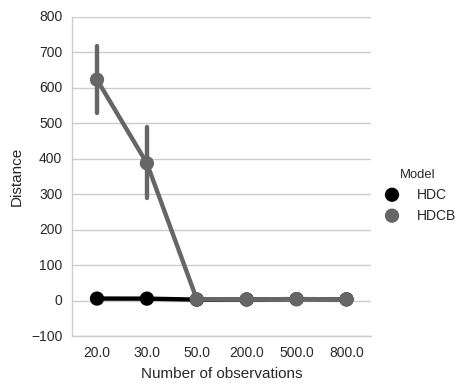
\includegraphics[width=\linewidth]{images/Eval-DC-KL-Distance.png}
    \caption{Kullback–Leibler divergence}
\end{subfigure}

\caption[DC, HDC Model Validation]{Measure of the distance between the learned probabilities and ground truth for models DC and HDB. The x-axis represents the different observations size.}
\label{fig:eval-B-KL-evaluation}
\end{figure}

Distances between the learned and the ground truth probabilities, learned using increasing number of observations is depicted in Figure~\ref{fig:eval-B-KL-evaluation}. The left plot is the Bhattacharyya distance while the right plot is the KL divergence. We can observe that with increasing number of observations the distance is getting reduced. With around 50 observations both the models  completely converged with the ground truth.  

From the figure we can also conclude that when the observations are very few the HDC model performs better than the DC model. This validates, that when there are some time periods which don’t have enough observations the hyper prior added in hierarchical model shares information between these time periods. HDC model performs better than DC model when the observations are few but as the observations increase there is no considerable difference in their learnings.

\section{Model Accuracy}

We have validated the working of the models on synthetic dataset in this section we validate HDC model on real world dataset. The aim of the experiments is to learn user location preferences on real world dataset. We employ two methods for evaluating the performance of HDC model. In addition to the traditional \emph{accuracy} measurements, we also evaluate the models based on the \emph{mean time to find the person}.  In the following section we explain the data collection procedure, data to information procedure and then the two evaluation methods.
 
\subsection{Aruba Dataset}
In our thesis, we have used a  publicly-available  dataset Aruba, published by the Lincoln Center for Autonomous Systems (LCAS). The dataset is of a person's location in a home collected at a smart apartment by the Center for Advanced Studies in Adaptive Systems (CASAS) \cite{aruba} .

The testbed where the dataset was collected is a  three-bedroom apartment located on the Washington State University that is part of CASAS smart home project \cite{aruba}.  The dataset consist of the location of a person in the home per second. The dataset was collected for over 118 days.


\begin{figure}
    \centering
    \begin{subfigure}[b]{0.4\textwidth}

        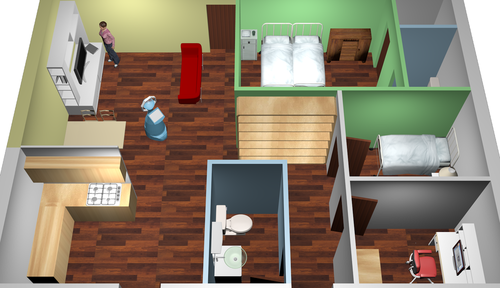
\includegraphics[width=\textwidth]{images/aruba-flat.png}
        \caption{Aruba apartment visualization}
        \label{aruba}
    \end{subfigure}
    ~ %add desired spacing between images, e. g. ~, \quad, \qquad, \hfill etc. 
      % (or a blank line to force the subfigure onto a new line)
    \begin{subfigure}[b]{0.5\textwidth}
        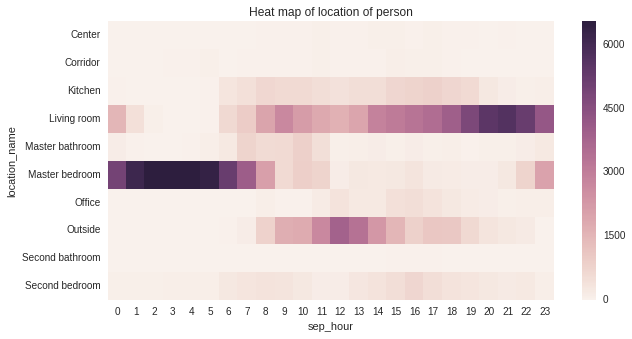
\includegraphics[width=\textwidth]{images/aruba-data.png}
        \caption{Heatmap}
        \label{fig:eval_gt}
    \end{subfigure}

    \caption[Aruba apartment visualization]{Aruba apartment visualization \citep{krajnik_wheres_2015} and Aruba dataset heatmap . In the heatmap, the y-axis are the locations of the home, x-axis are the hours of the day. The intensity of the colour in each box indicates the number of times the person is present in that location. Higher the intensity means more time is spent by the person in that location at that time.}
    \label{aruba-visual}
\end{figure}

As shown in Figure~\ref{aruba}, the smart apartment test bed includes three bedrooms, one bathroom, a kitchen, and a living / dining room.  The apartment is equipped with motion sensors distributed approximately 1 meter apart throughout the space. The Aruba dataset was extracted from these motion sensor dataset provided by CASAS. The dataset contains the location of a person in the apartment every minute for 16 weeks.

We process the dataset and  order it as a  $(hour,location)$ tuple. We visualize the dataset as a heatmap over locations distributed over different periods. As explained in chapter~\ref{cha:approach}, we try to learn daily patterns by dividing the observations into per hour periods. As we can see there are some prominent patterns present which can be learned. For example the usage of the bedroom, living room, outside and kitchen.


\subsection*{Sparsification}
Aruba dataset is a large dataset as compared to an person location dataset we assume the robot will be able to generate. The Aruba dataset has recordings of every minute for 118 days, which is 161280 readings.
On the contrary the assumed dataset which will be collected by the robot by autonomously roaming in a home will be just 3-5 readings per day.
So for simulating the sparsity in the object location dataset we will sparsify the ARUBA dataset by random selecting only selecting 3-5 readings each day.

After sparsification by randomly selecting 5 readings per day the dataset is reduced to 590 observations. The heatmap the of the sparsified dataset is shown in Figure~\ref{aruba-reduced-hist}. 



\begin{figure}
    \centering
    \begin{subfigure}[b]{0.55\textwidth}
    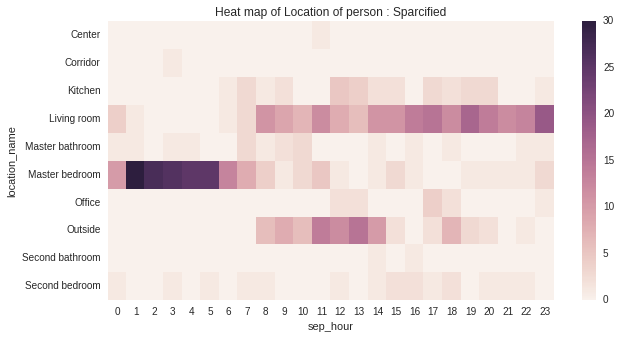
\includegraphics[width=\textwidth]{images/aruba-reduced-heatmap.png}

    \caption{}
        \label{aruba_sparse}
    \end{subfigure}
    ~ %add desired spacing between images, e. g. ~, \quad, \qquad, \hfill etc. 
      % (or a blank line to force the subfigure onto a new line)
    \begin{subfigure}[b]{0.4\textwidth}
    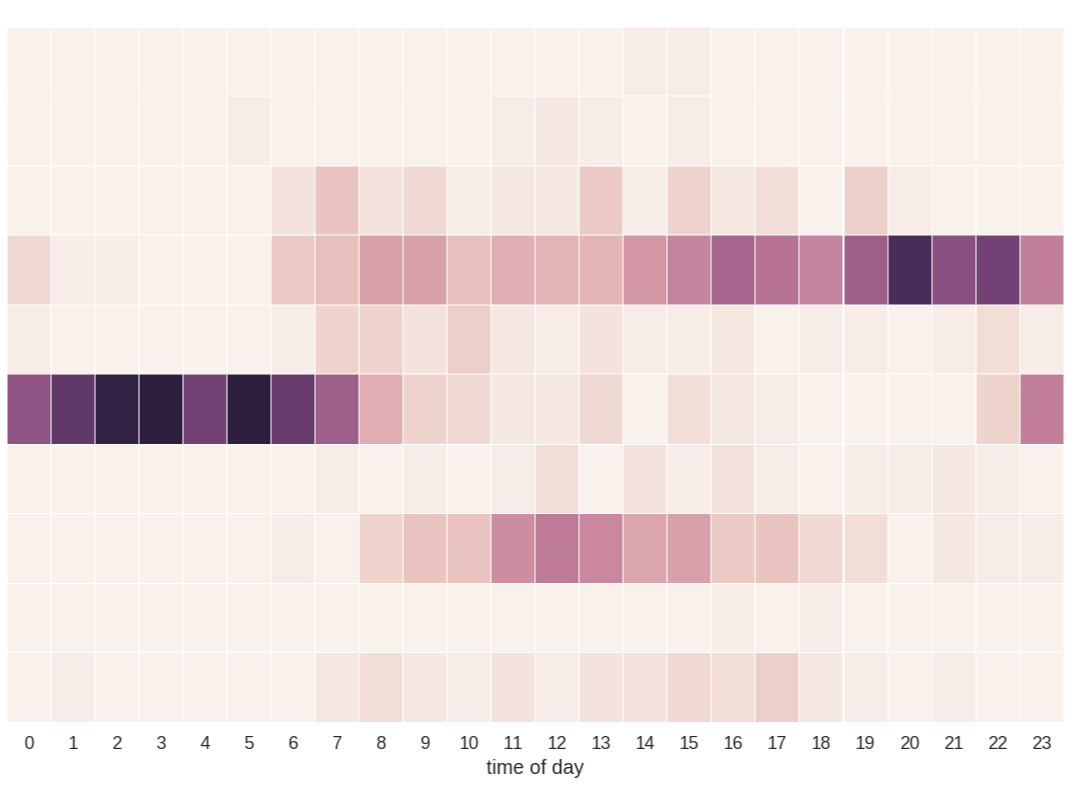
\includegraphics[width=\textwidth]{images/learned-aruba.png}
        \caption{}
        \label{fig:learned_aruba}
    \end{subfigure}
    \caption[Aruba sparcified dataset vs learned model  heatmap]{(a)Aruba sparcified dataset heatmap :The y-axis are the locations of the home, x-axis are the hours of the day. (b) Learned distribution using HDC model.} 
\label{aruba-reduced-hist}
\end{figure}

\FloatBarrier


\subsection{Comparison With State-Of-Art Machine Learning Algorithms}

In this section we evaluate the predictive capabilities of our learned model. The accuracy of the predictions are measured and then compared with other state of the art machine learning algorithms. Two state-of the-art machine learning algorithms: Support Vector Machine (SVM)\citep{boser1992training, cortes1995support} and Random Forest \citep{breiman2001random, geurts2006extremely}. Scikit-learn \citep{sklearn_api} implementation of the algorithm were used for testing.

The goal of learning users location preference is to predict the location of the user based. We interpret the problem as a supervised machine learning with known input and outputs.In supervised learning the data comes a finite learning set $L =  (X, y)$ where, $X = input\ values$ and $y = output\ values$. 
For our problem statement the input is single feature, the time of the observation $X = [time]$, the output is the location of the person $y=[location]$

The learning was conducted using training set of different sizes, ranging from 0.0003\% (484 observations i.e. around 5 observations per day by the robot) to 0.2\% (32256 observations) of the dataset. The remaining data was used as testing set. The accuracy score for the classification is plotted in Figure~\ref{fig:SVM_vs_DCM}. 

\begin{figure}
    \centering
    \begin{subfigure}[b]{0.44\textwidth}
        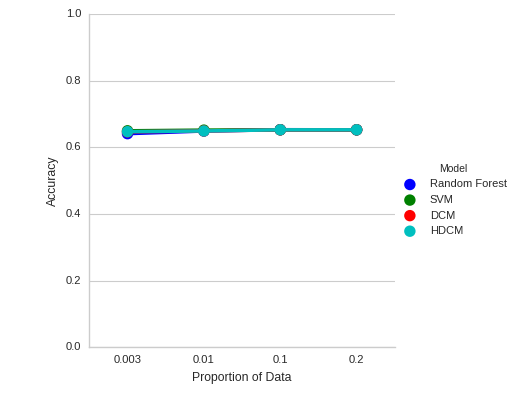
\includegraphics[width=\textwidth]{images/svm_vs_HDCM.png}
    \end{subfigure}
    \begin{subfigure}[b]{0.44\textwidth}
        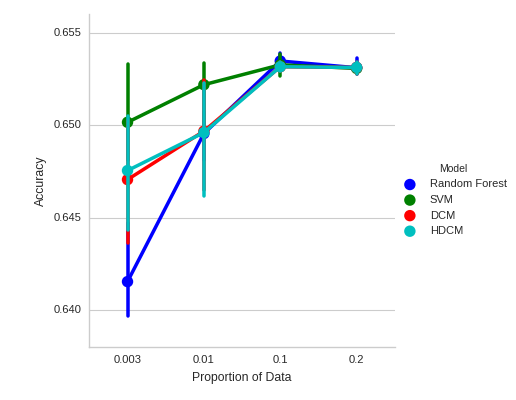
\includegraphics[width=\textwidth]{images/svm_vs_HDCM_zoomed.png}       
    \end{subfigure}
    
    \caption[Comparison with SVM and Random Forest]{ Comparison with SVM and Random Forest. The right plot is the zoomed view between 0.64 to 0.65}
    \label{fig:SVM_vs_DCM}
\end{figure}

As per the accuracy plot there is no considerable difference between the accuracy of  SVM, Random Forest, DC and HDC . Also the maximum accuracy is around 0.64\% , which doesn’t increase even with increasing number of observations. 


\subsection{Search time evaluation}
The models were also evaluated on the basis of the \emph{search time} to find the person. As mentioned above the goal of modelling human presence is to predict the persons location and reduce the time of search. Thus by calculating the time required to search the person based on the predictions of the model we can evaluate the performance of the learning \citep{krajnik_wheres_2015}.

\cite{krajnik_wheres_2015} in their seminal paper have proposed a path-planning search algorithm. This algorithm is used to determine the shortest path to be taken by the robot based on each locations probability. Thus it goes first to the most probable location first, then to other locations in decreasing order of the probabilities. \cite{krajnik_wheres_2015} solve the problem of learning preference of user location using temporal models. Two temporal models, frequency map enhancement  model  (FreMEn) and periodic Gaussian model (PerGaM) were used to learn the location preferences. 

We compare our developed model HDC along-with the FreMEn model based on the search time. A 'Static' model represented by static probability is used as a reference. Out of the 16 weeks of the Aruba dataset, first 4 weeks were used by \cite{krajnik_wheres_2015} to learn the models and last 12 weeks were used for testing. While in our case we learned using the sparse Aruba dataset  (~550 observations), and testing using same the last 12 weeks as above.

\begin{figure}[htp]
\centering
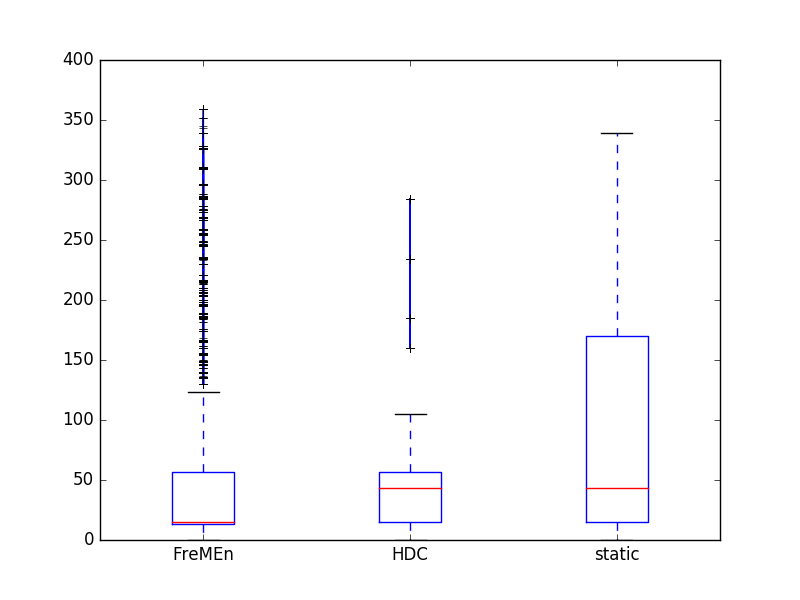
\includegraphics[width=0.5\textwidth]{images/box_plot_fremen_hdc.png}
\caption[Search time evaluation]{Search times for different models}
\label{fig:search_time}
\end{figure}

The search results were compared with FreMEn model and Static model. In static model the robot has no knowledge about the person locations and has a pre defined search path. 
The average time required to search for a person was reduced using the HDC model search and temporal model search as compared to the static model. This can be observed in Figure~\ref{fig:search_time}. While the difference in the average between the static and the HDC model is very less, the quartile of HDC is fairly reduced. The quartile reduction was mainly due to the fact that 90\% of the time the HDC model was able to search within the first 4 predictions of the person i.e. 92\% the person was located within the first 4 predictions. 

The average time of the FreMEn model is very less as compared the HDC model. Thus we can conclude that FreMEn has better performance. But we can observe that FreMEn has a long whisker, which was explained as short-term absences of persons at the expected locations \citep{krajnik_wheres_2015}. However these whiskers are missing with the HDC model.

\section{Discussions}

In this chapter, we presented probabilistic model to learn user location preferences.  In chapter \ref{chapter:occupancy} the models captured knowledge about each location separately, while in this chapter the models are able to capture knowledge about multiple locations in a single model. 

In a set of experiments on synthetic dataset, we found that our model is capable of learning underlying patterns in user preferences. In first set of experiments we did a sanity check of our learning by visualizing the learned probability. Then we compared DC and HDC model and validated that addition of a hyper-prior improves learning when the observations are sparse. Furthermore, we evaluated the performance of the models predicting capability on a real world dataset, where the predictive accuracy results were around 63\% . The reason for such low accuracy result even with increasing number of dataset, can be explained by \cite{Bishop20120222} reasoning of ``Large" dataset. The author explains that learning is bad in some computationally large  (size) dataset as their statistical size in relation to the model is small. The Aruba dataset is likely that it is statistically small dataset.

We compared the search time required by the robot to find the person in the home. The average search time of the model is reduced than the static search timings, but the median search time is very high as compared to the temporal model, FreMEn \citep{krajnik_wheres_2015}. One of the reasons can be that our models learns on a hour level sparse dataset while FreMEn was learned at minute level dataset. 

The mean time required to search the person is lower as compared to the search with no knowledge about user preferences, we can conclude that by learning user preferences the robot can make informed decisions that decrease the search time.

% section   (end)





